\chapter{EC2}\label{ch:ec2}

\subsection{AWS Setup}\label{subsec:aws-setup}

After the configuration of the VPC and subnets was completed, the initial deployment of the web app began through
setting up EC2.
This AWS service allows for scalable computing capacity through the use of a virtual computing environment hosted in the
cloud~\parencite{aws2022ec2}.
The web app will be stored on an EC2 instance of Amazon Linux, known as Amazon machine images (AMIs), which wil then be
launched through a docker container stored on the app.

\begin{figure}[!htbp]
    \centering
    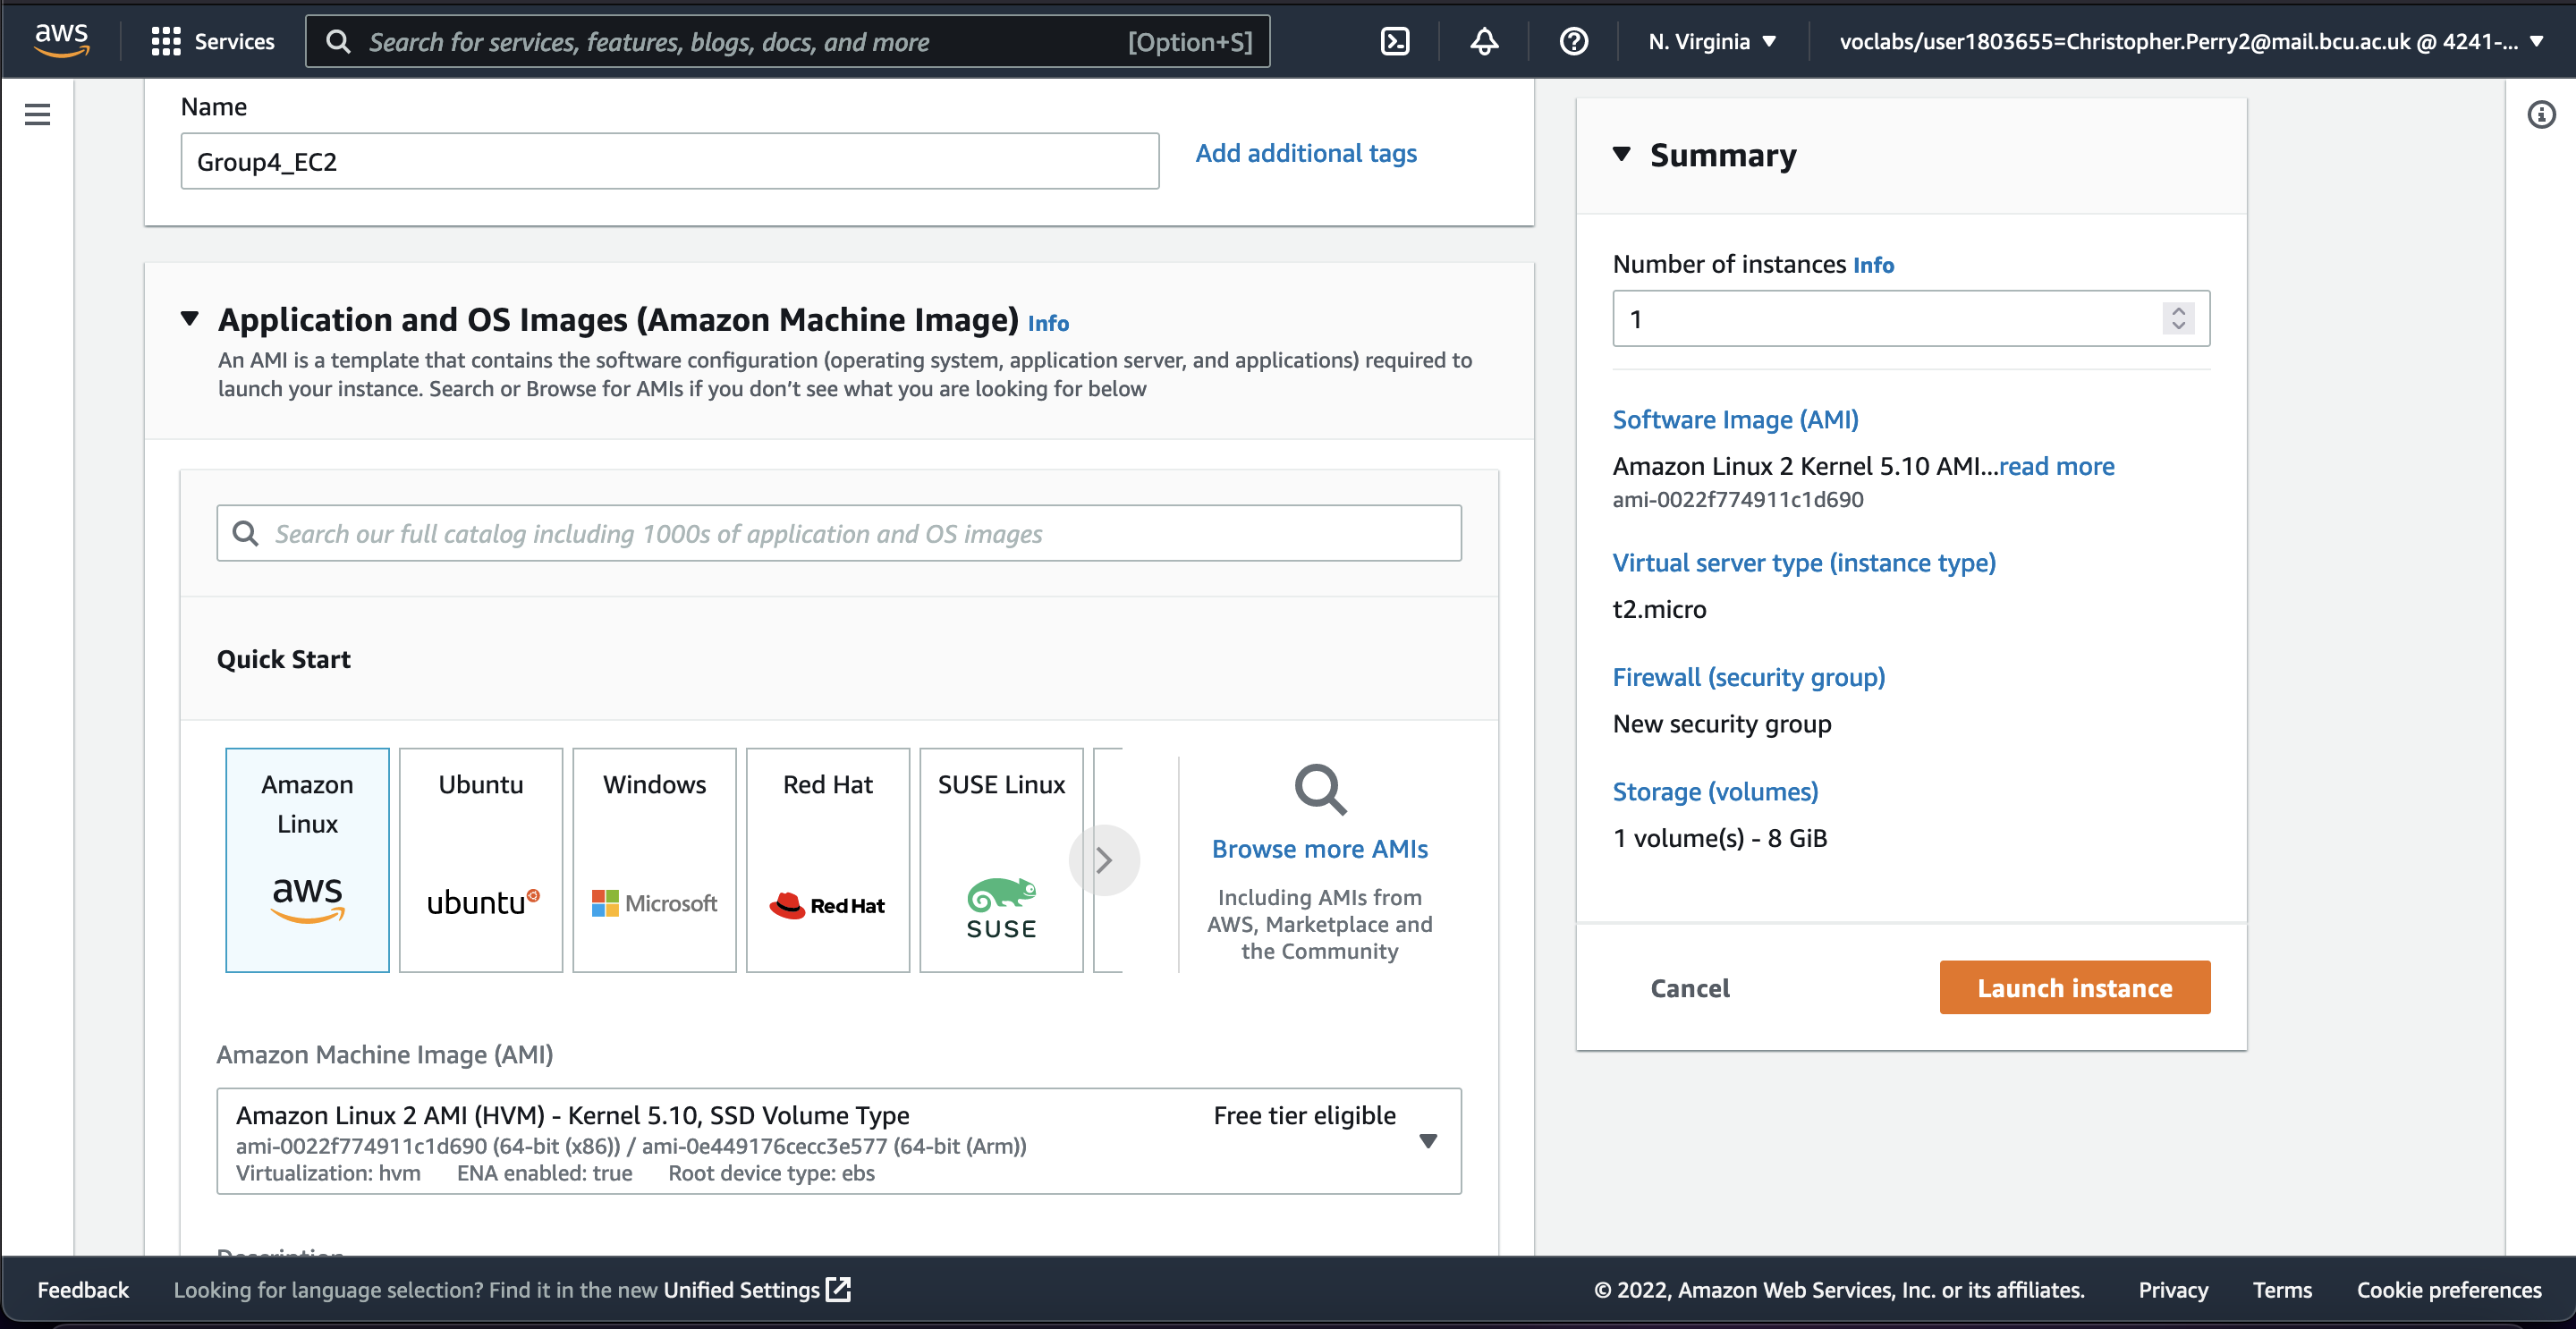
\includegraphics[scale=0.3]{resources/ec2/create-instance-application-and-os-images}
    \caption{Selection of EC2 OS Image.}
    \label{fig:ec2-os}
\end{figure}

Figure~\ref{fig:ec2-os} details the selection of the Operating System (OS) that will be used for the EC2 instance.
The \textit{Amazon Linux 2} AMI was selected, as it is already configured with Linux and does not need any more setup.

\clearpage

Now that an AMI has been chosen, the specific instance type that will be used within this AMI can be selected.
It was decided that the instance type of \textit{t2.micro} would be used, as it contains only 1GB of Random Access
Memory (RAM).
The selection of this can be found in Figure~\ref{fig:ec2-instance}.

\begin{figure}[!htbp]
    \centering
    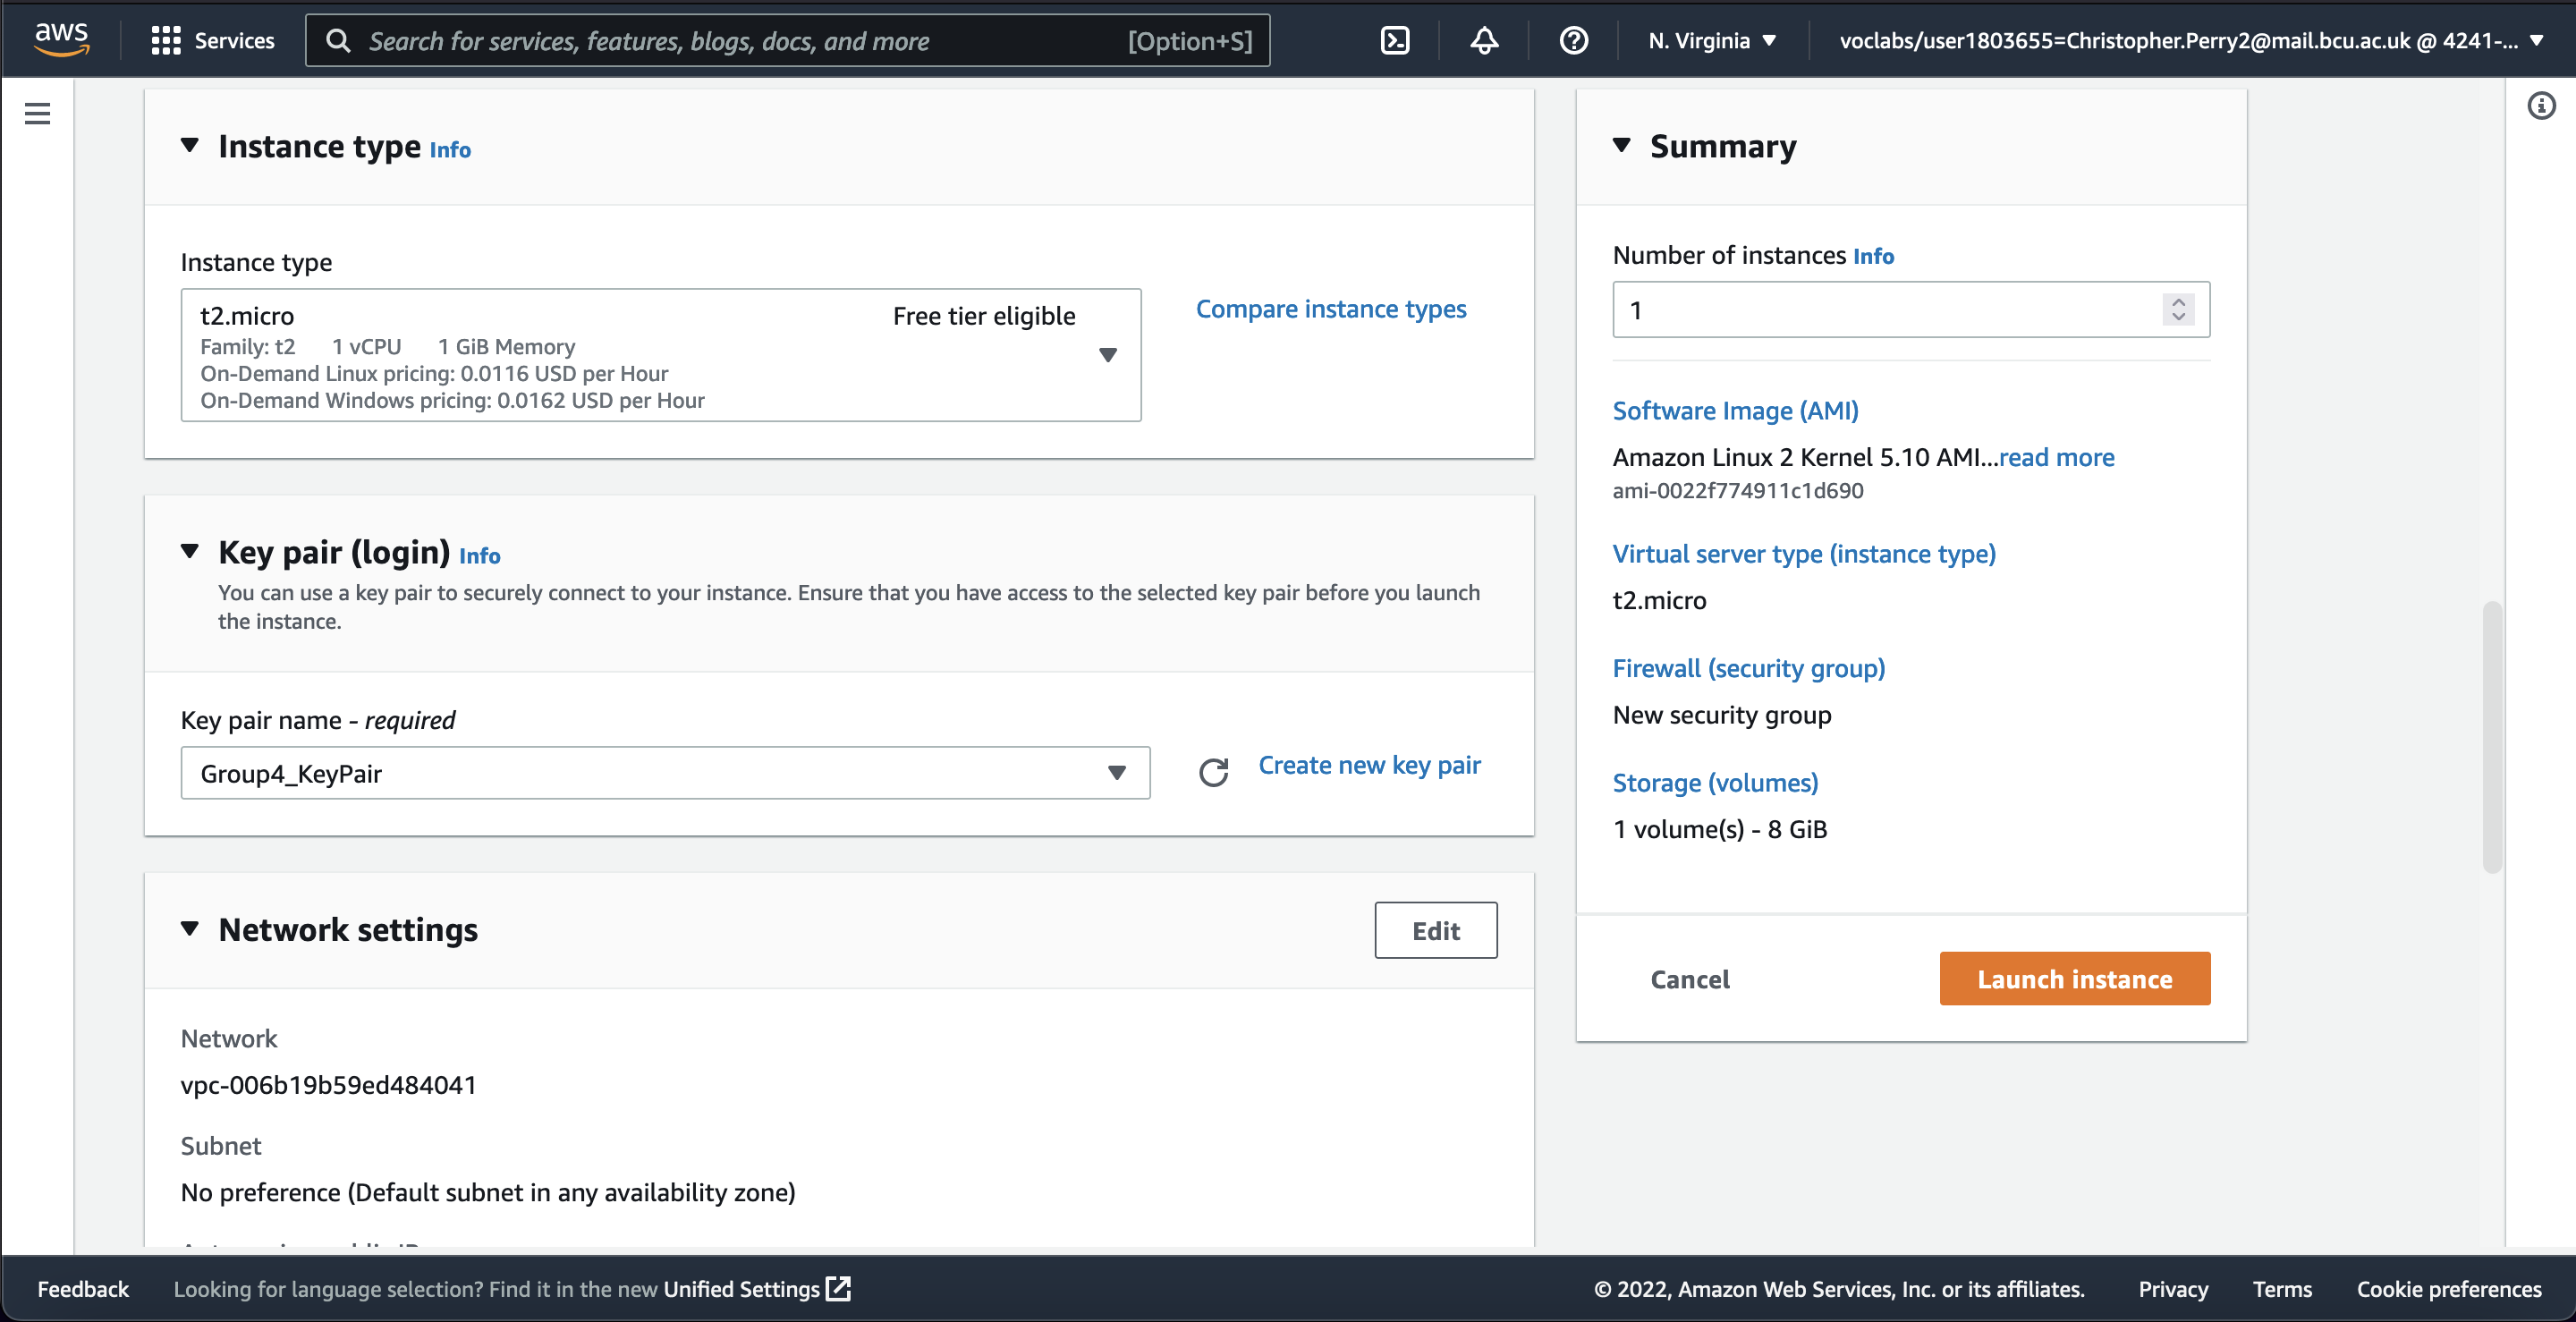
\includegraphics[scale=0.3]{resources/ec2/create-instance-instance-type}
    \caption{Selection of EC2 Instance.}
    \label{fig:ec2-instance}
\end{figure}

A key pair will allow for the ability to sign in to the EC2 instance with a unique set of login credentials, heightening
the security of the project.

The next stage of the setup process was to set up networking for the EC2 instance, in order for the web app to work with
Docker to download relevant containers from DockerHub, which will allow a Laravel instance to be initialised, as
discussed in Section~\ref{ch:web-app}.

\begin{figure}[!htbp]
    \centering
    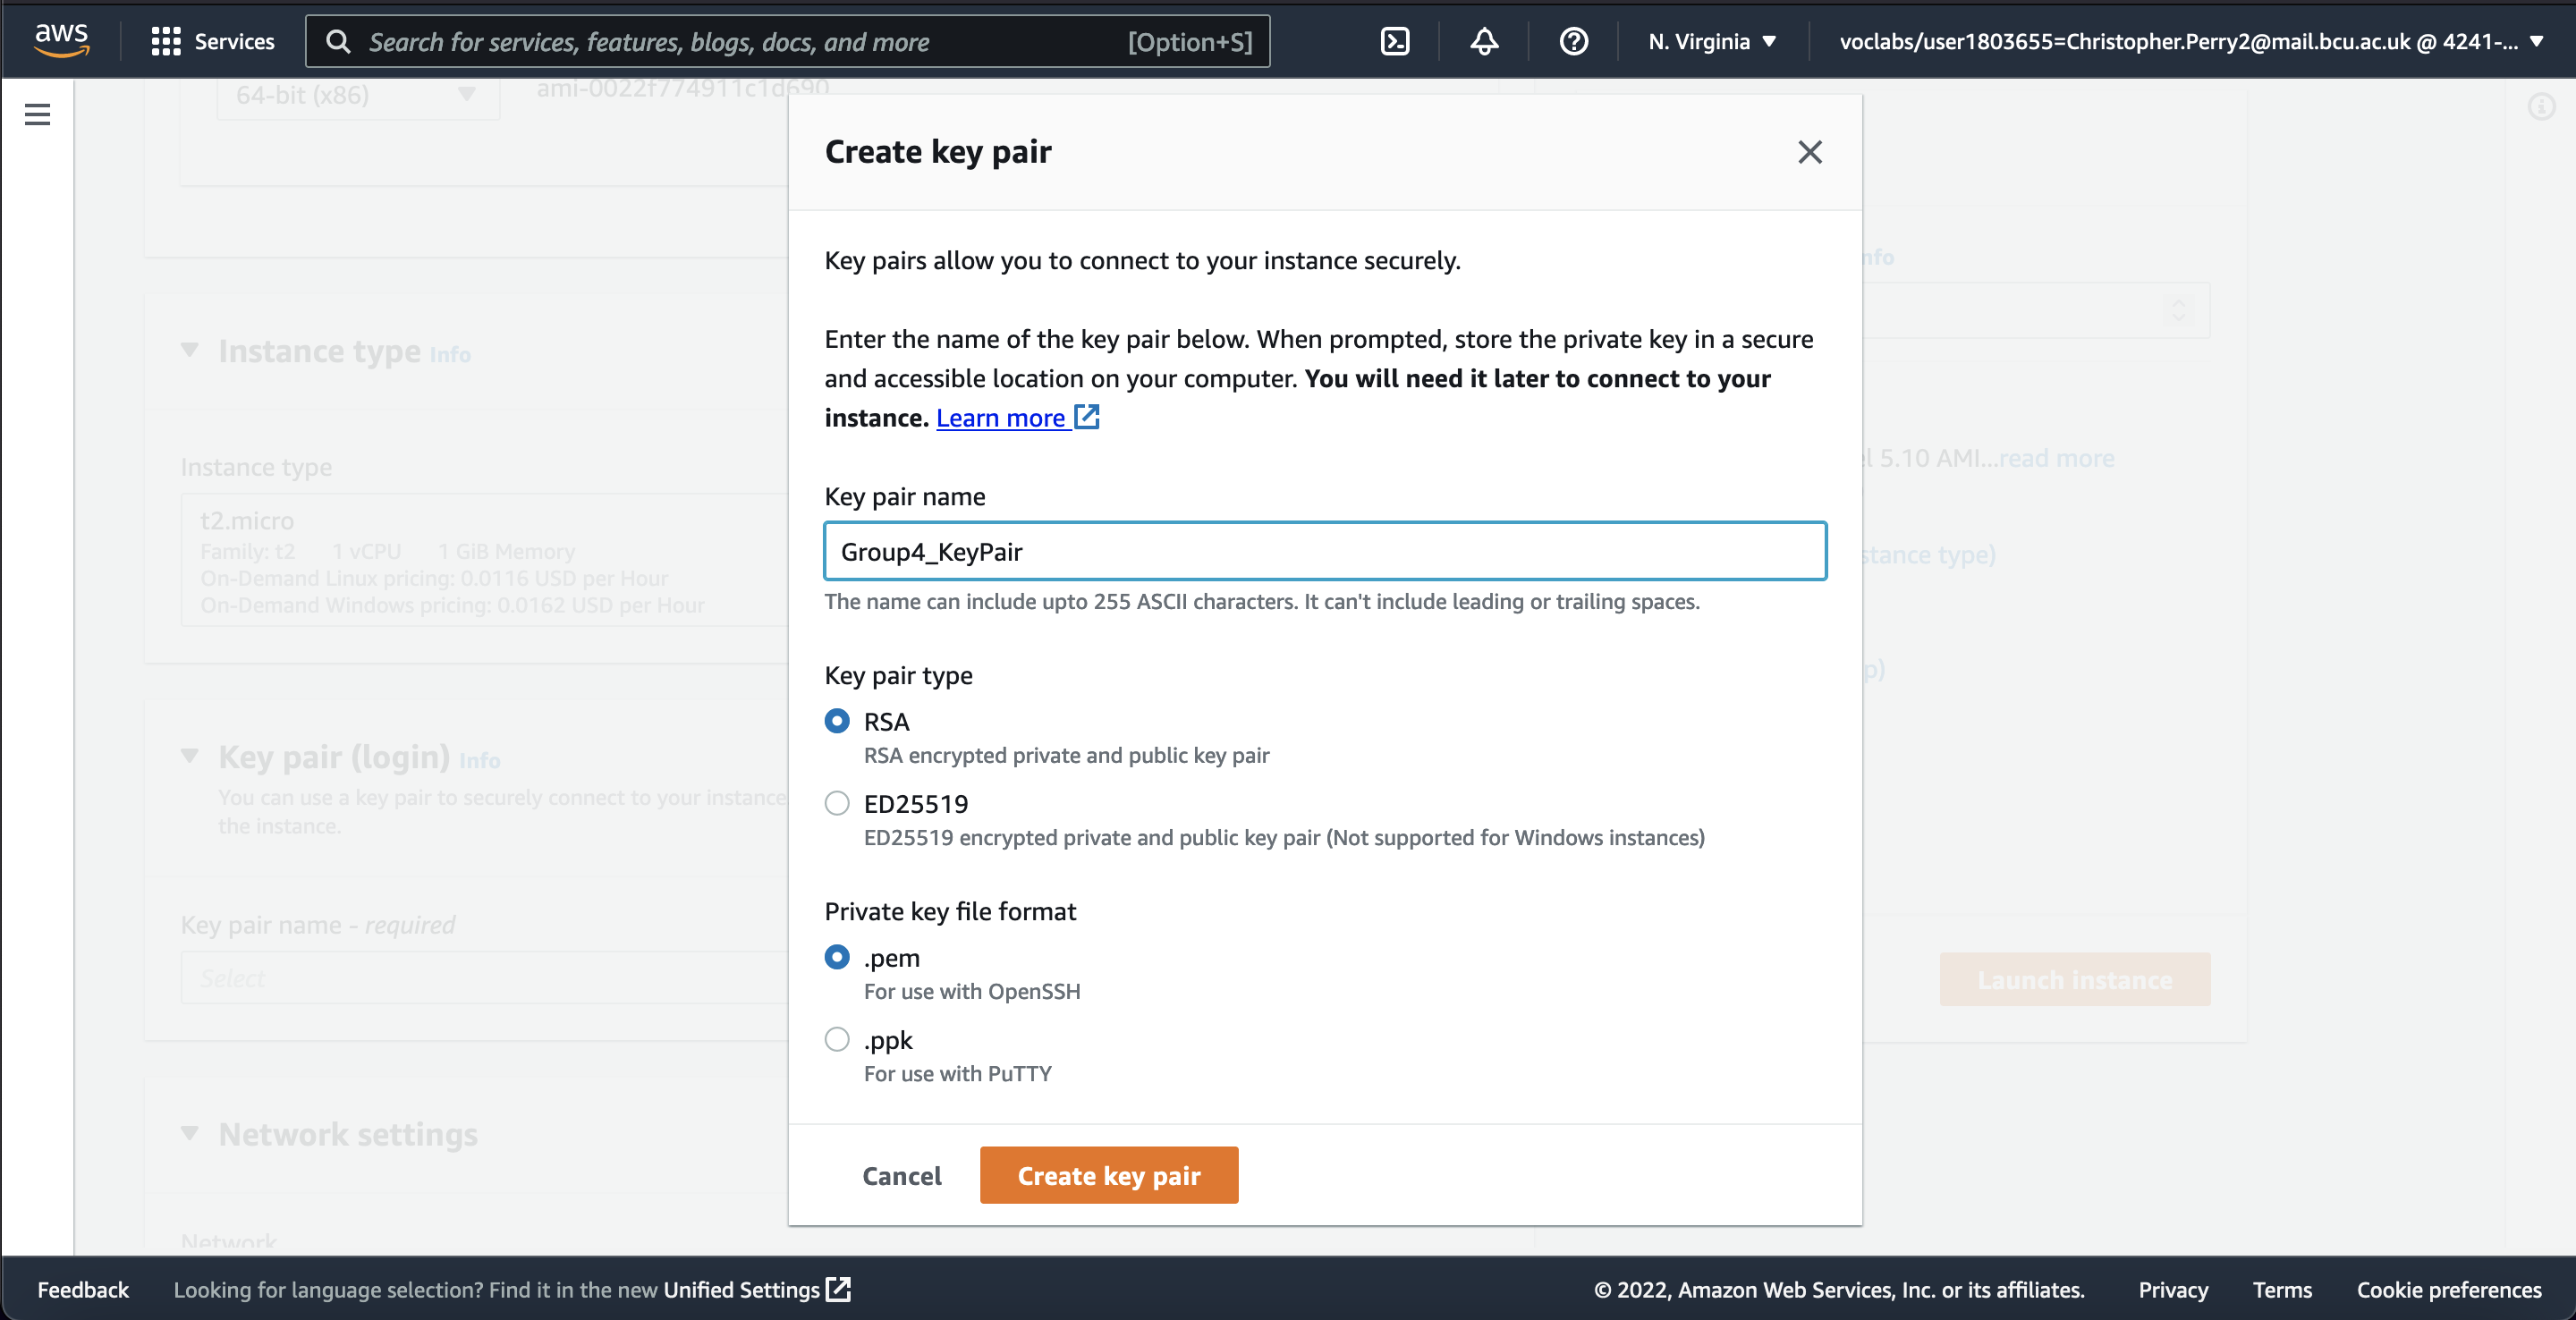
\includegraphics[scale=0.3]{resources/ec2/create-key-pair}
    \caption{Selection of EC2 Keypair.}
    \label{fig:ec2-keypair}
\end{figure}

This process can be seen in Figure~\ref{fig:ec2-keypair}.

The instance is assigned the VPC created in Section~\ref{ch:vpc_subnets}, where it is assigned a subnet in the same
availability zone of us-east-1.

\begin{figure}[!htbp]
    \centering
    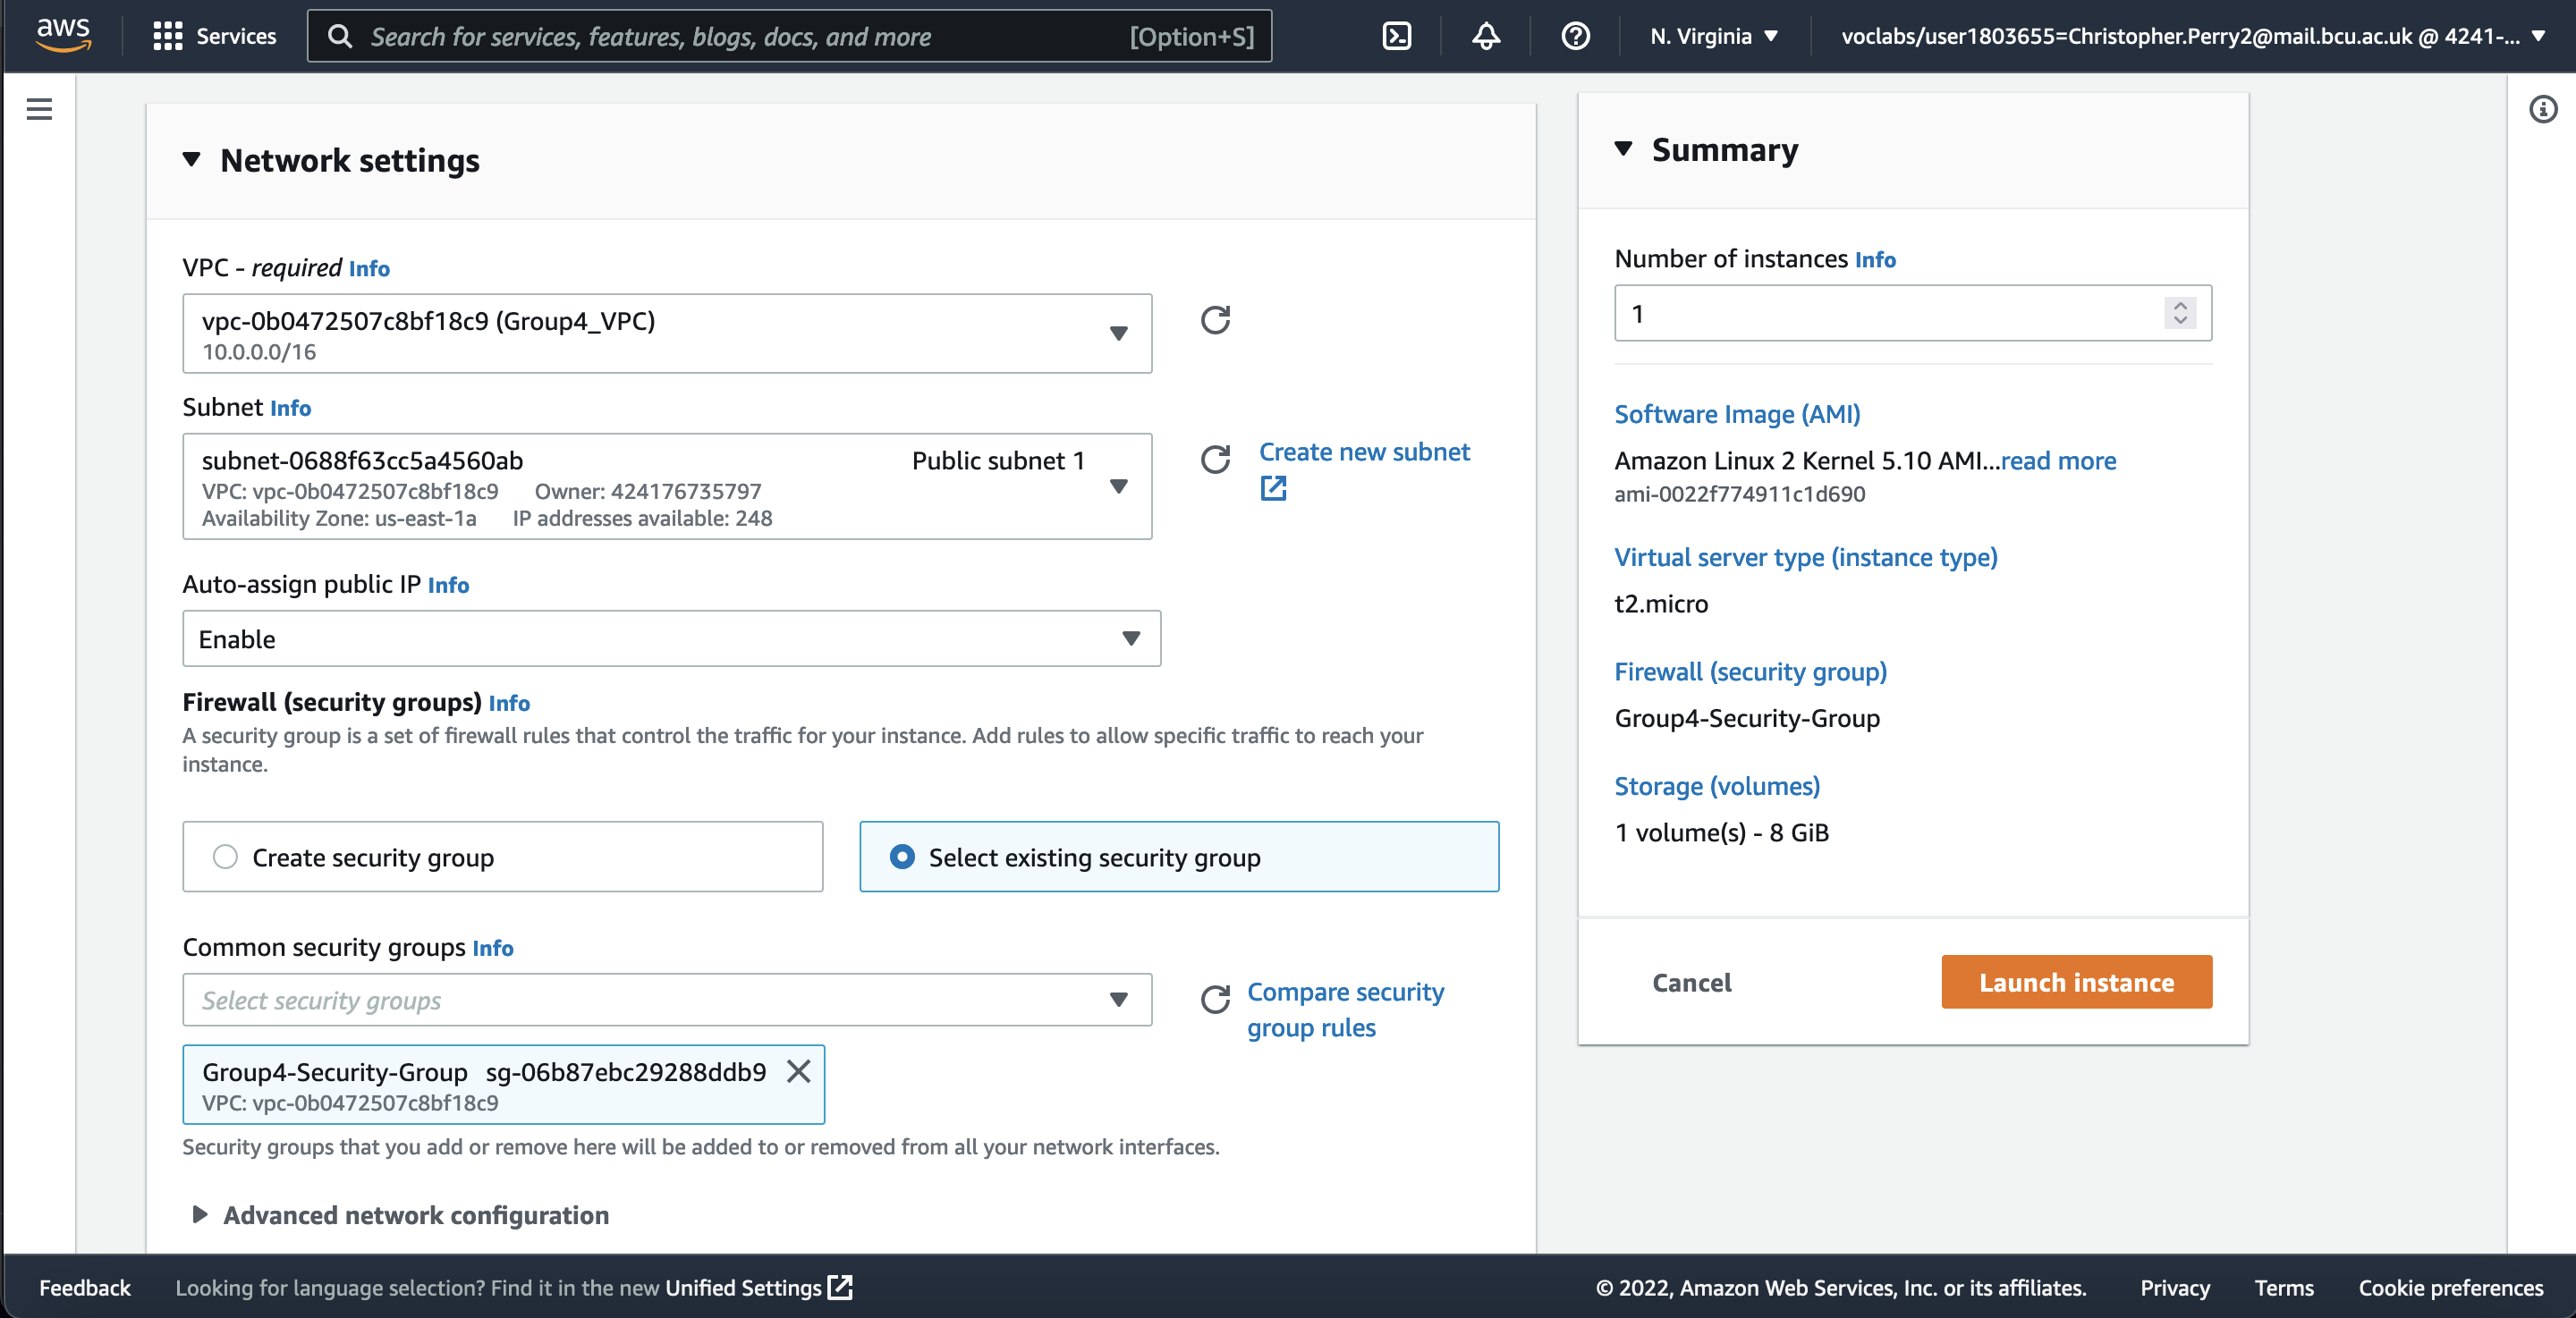
\includegraphics[scale=0.3]{resources/ec2/create-instance-network-settings}
    \caption{Selection of EC2 Networking options.}
    \label{fig:ec2-networking}
\end{figure}

\begin{figure}[!htbp]
    \centering
    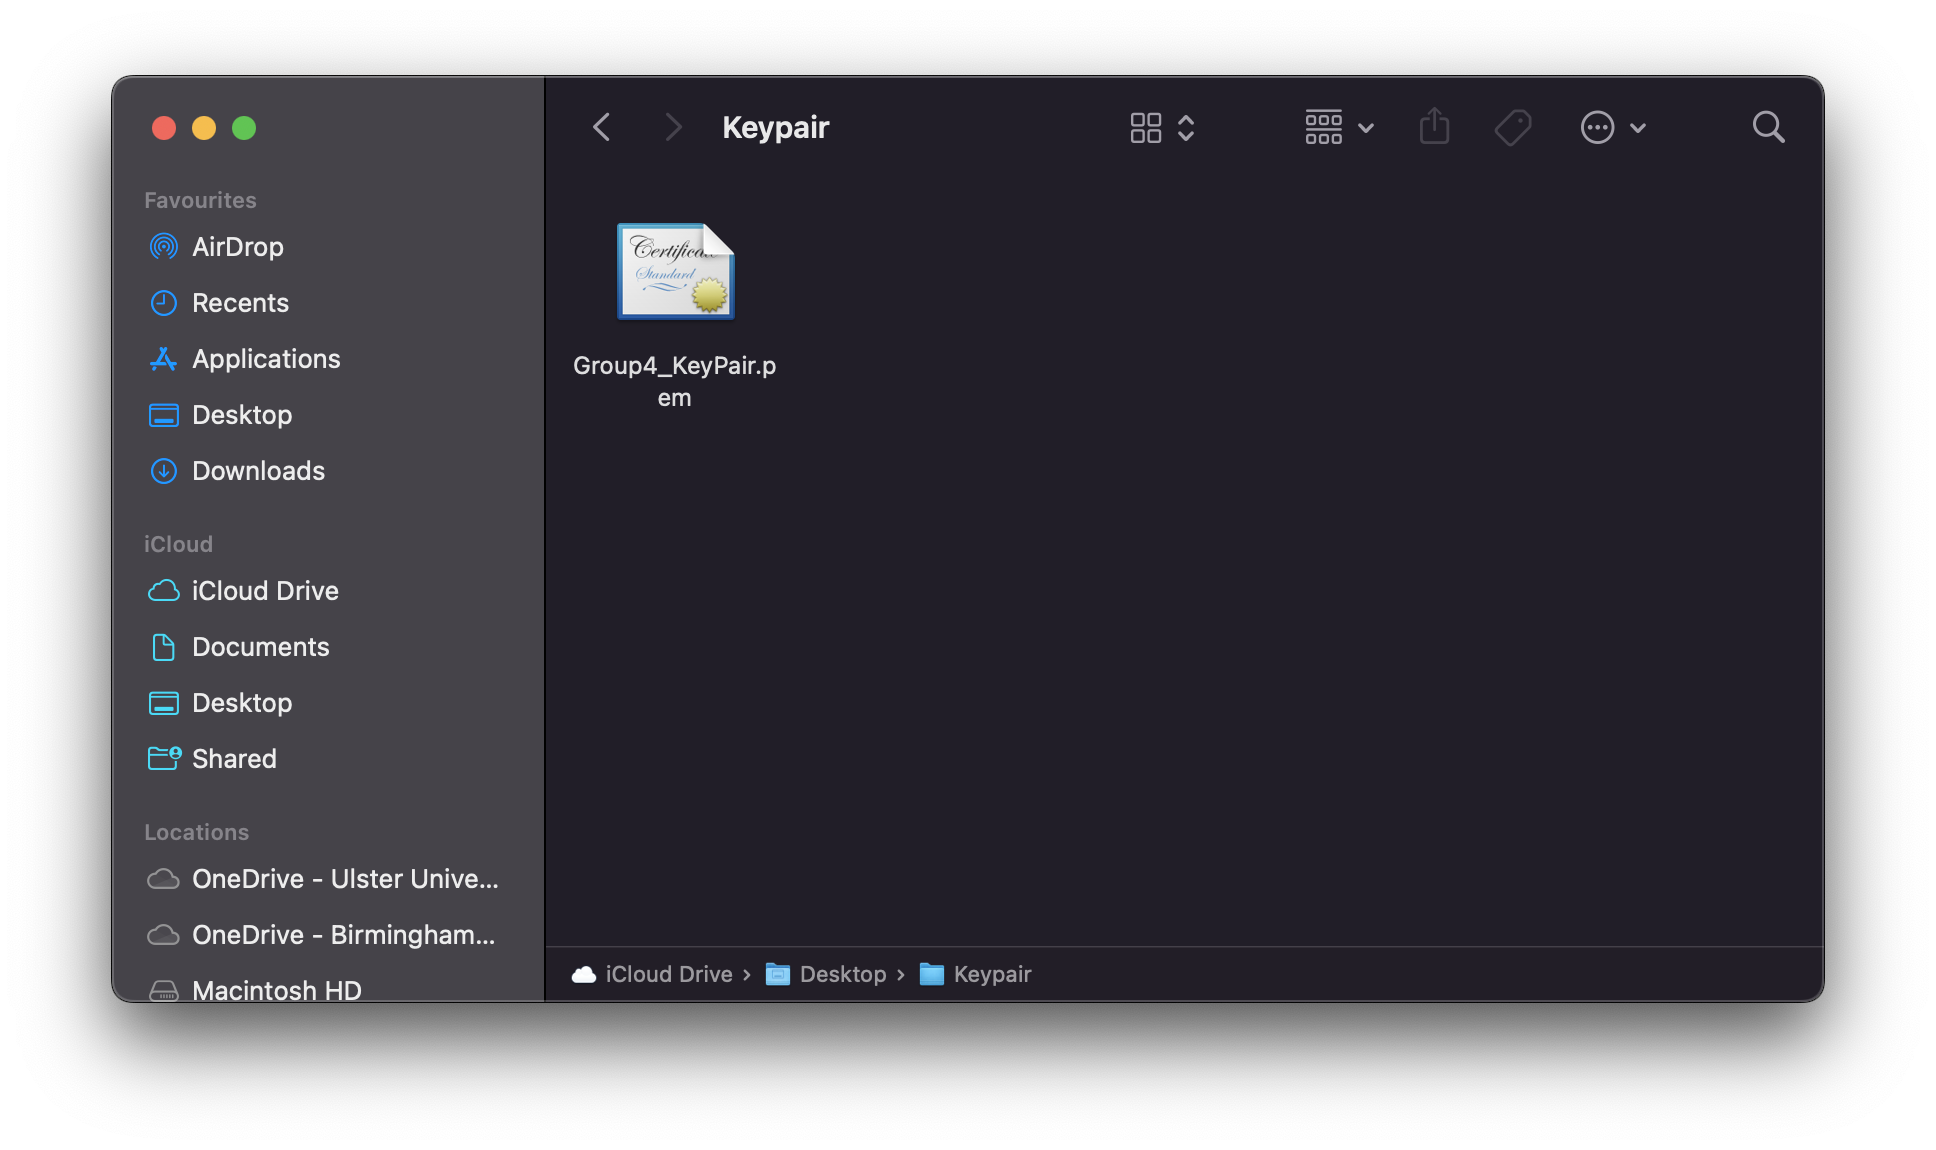
\includegraphics[scale=0.3]{resources/ec2/keypair}
    \caption{Generated EC2 Keypair in the \mintinline{sql}|.pem| format.}
    \label{fig:keypair}
\end{figure}

This setup can be seen in Figure~\ref{fig:ec2-networking}.
An EC2 keypair is then generated in the \mintinline{sql}|.pem| format.

This is enough to comfortably run the web app without any issues.
Storage for the AMI was subsequently chosen.
It was decided that 8GB of storage would be used, as this is enough to run the web app and still provide leftover storage
for any system-critical tasks.

\begin{figure}[!htbp]
    \centering
    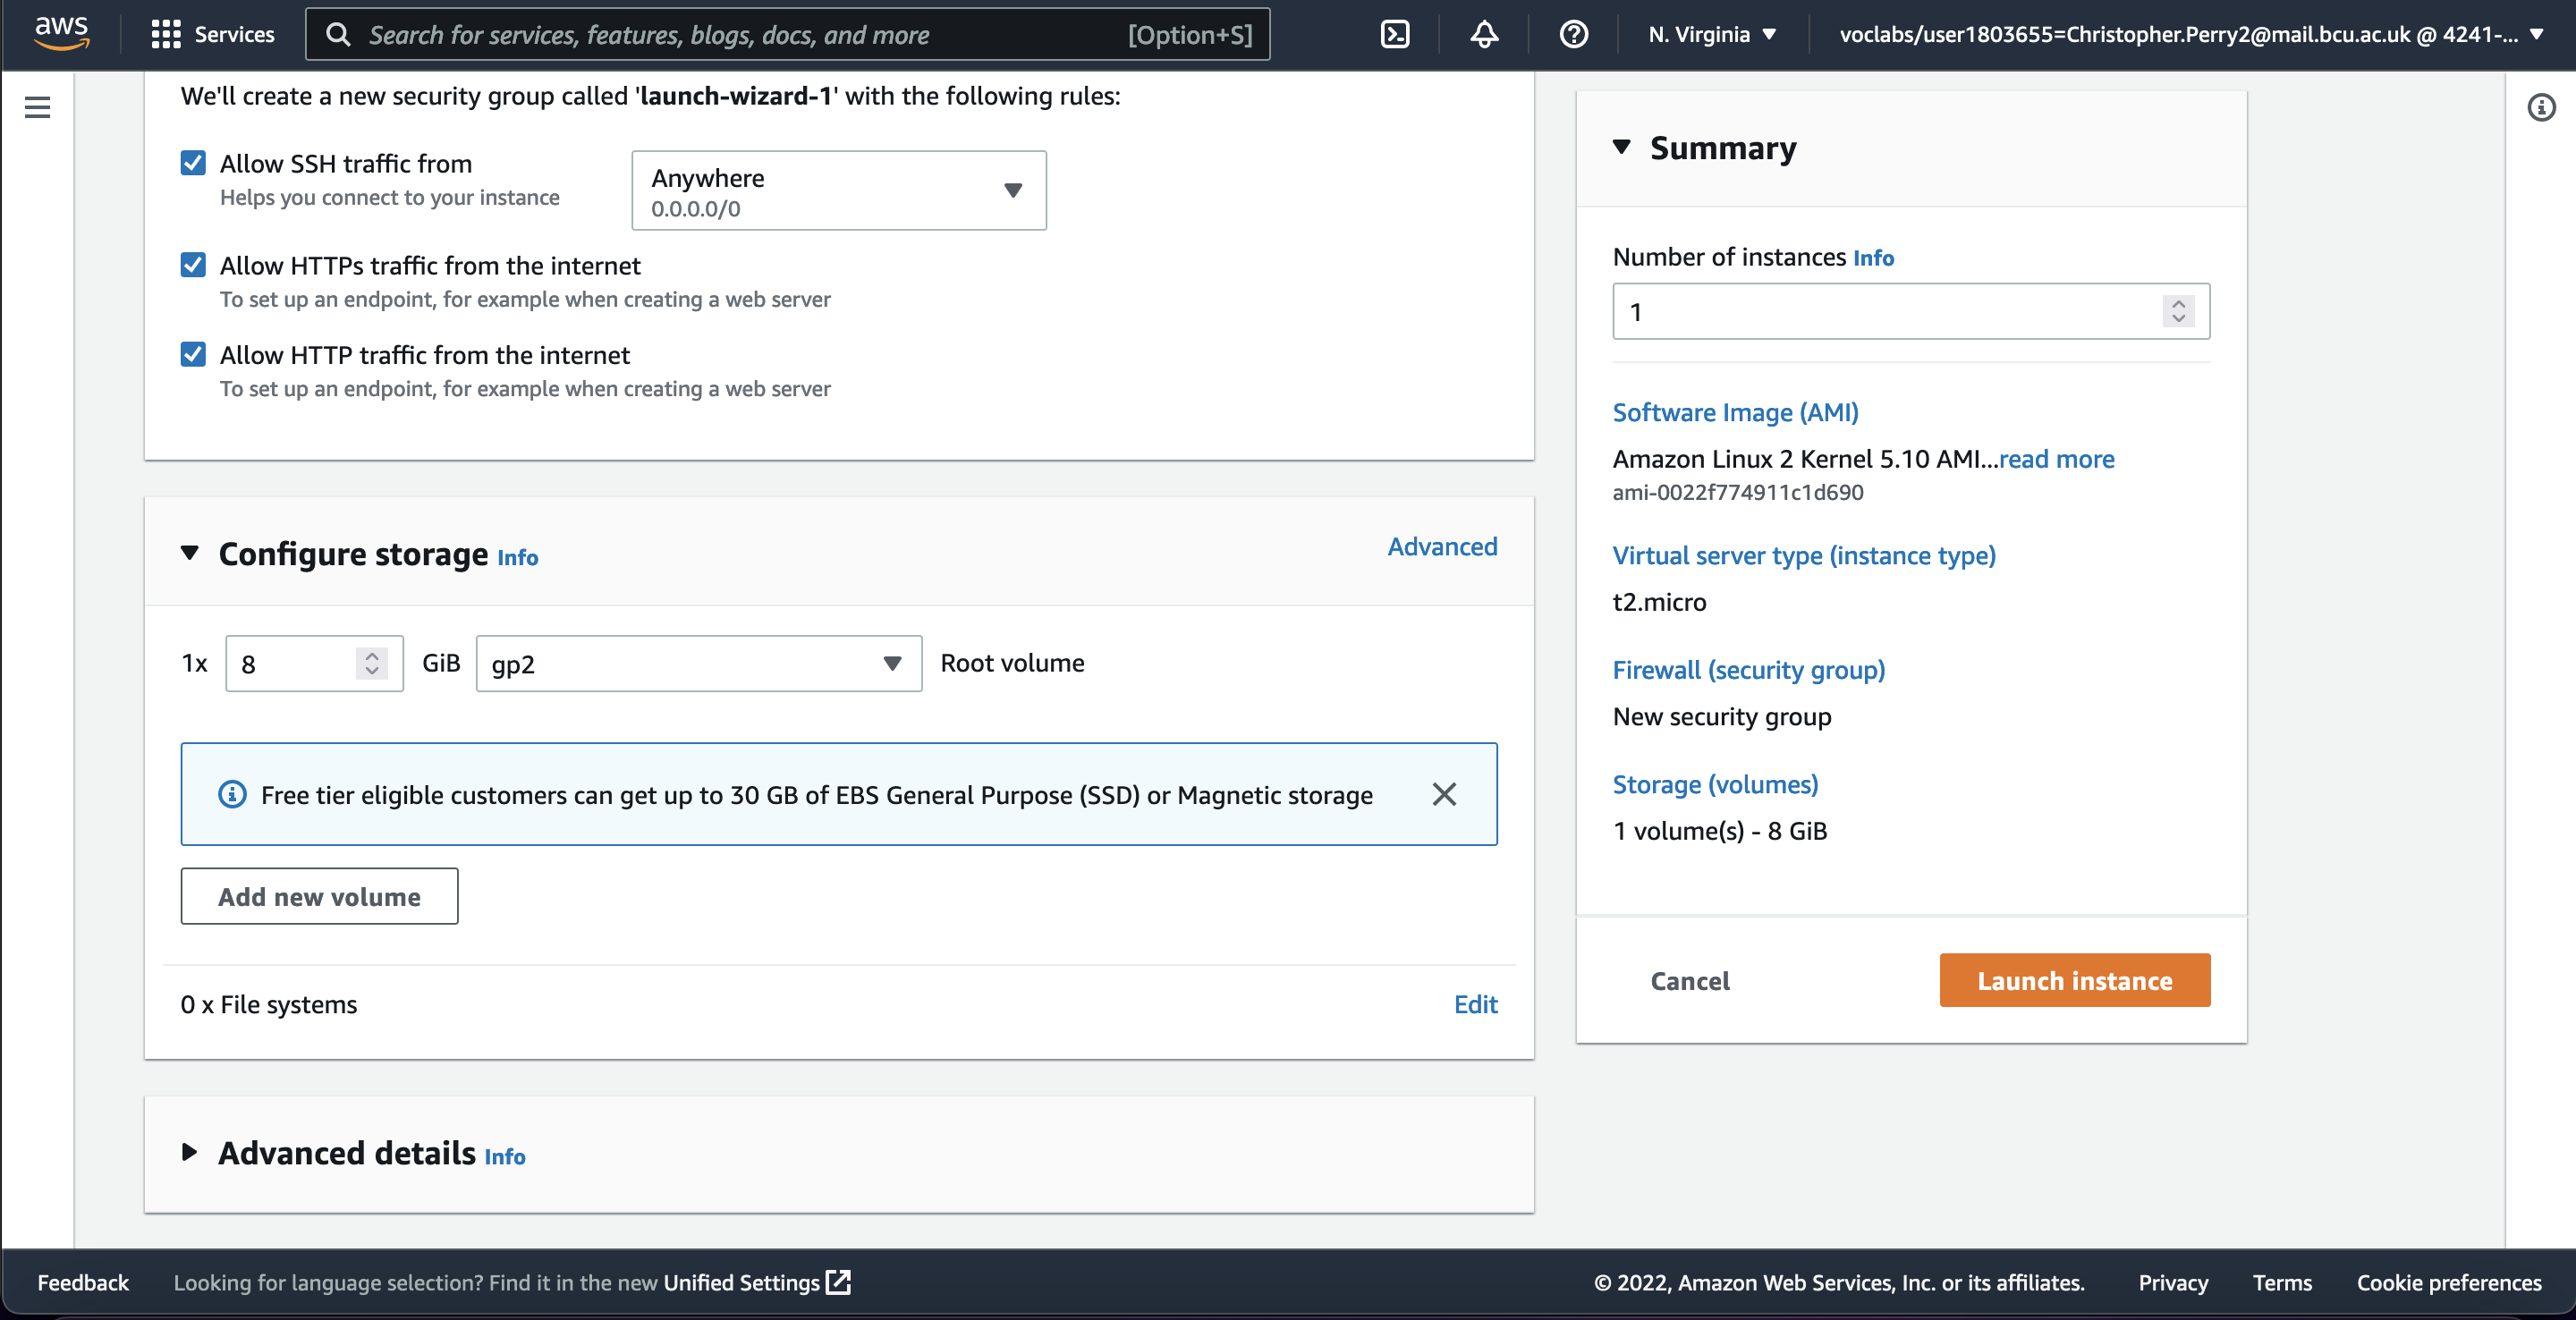
\includegraphics[scale=0.3]{resources/ec2/create-instance-configure-storage}
    \caption{Selection of EC2 Storage Configuration.}
    \label{fig:ec2-storage}
\end{figure}

The selection of these options can be found in Figure~\ref{fig:ec2-storage}.
In addition to this, the chosen options are eligible for "Free Tier", which means that it will use a limited amount of the
\$100 budget allocated for the project.


\subsection{Web app Setup}\label{subsec:webapp-setup}

The EC2 instance \mintinline{sql}|group4-ec2| is now live, and the webapp can be loaded onto it.
The instance is first logged in to through the use of the \mintinline{sql}|ssh| command, followed by the IP address of
the instance.

